\documentclass{article}
\usepackage[utf8]{inputenc}
\usepackage{tikz}
\usepackage{pgfplots}
\pgfplotsset{compat=1.18}

\title{LaTeX Environment Test with TikZ and pgfplots}
\author{Antigravity}
\date{\today}

\begin{document}

\maketitle

\section{Introduction}
This is a sample document to verify the LaTeX environment setup on Docker.

\section{TikZ Sample}
Here is a simple TikZ graphic:

\begin{center}
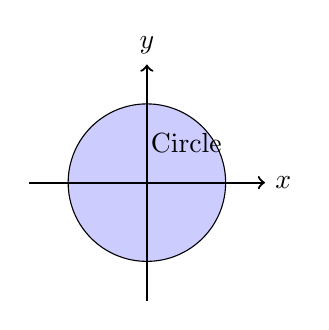
\begin{tikzpicture}
    \draw[fill=blue!20] (0,0) circle (1cm);
    \draw[->, thick] (-1.5,0) -- (1.5,0) node[right] {$x$};
    \draw[->, thick] (0,-1.5) -- (0,1.5) node[above] {$y$};
    \node at (0.5,0.5) {Circle};
\end{tikzpicture}
\end{center}

\section{pgfplots Sample}
Here is a simple plot using pgfplots:

\begin{center}
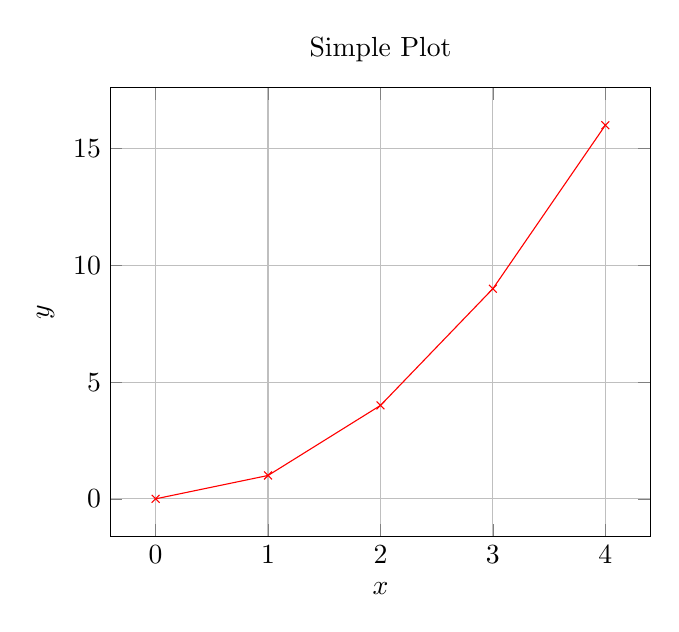
\begin{tikzpicture}
\begin{axis}[
    xlabel={$x$},
    ylabel={$y$},
    title={Simple Plot},
    grid=major,
]
\addplot[color=red, mark=x] coordinates {
    (0,0) (1,1) (2,4) (3,9) (4,16)
};
\end{axis}
\end{tikzpicture}
\end{center}

\end{document}
